\scanpage{71}
\mspage{324}

\deleted{We must therefore \unsure{have}}

\unsure{Henceforth} we \unsure{restrict} ourselves to the automorphisms
(\inserted{\unsure{actual or}} outer) of $\widehat{\Pi}_{0,3}$
which \unsure{respect} the loop structure, and \unsure{commute} with
$\mathfrak S_3$ (as outer actions)
--- which \unsure{correspond} to the automorphisms
\inserted{(\unsure{actual or outer})} of
$\widehat{\mathfrak S}_{0,3}^{+}$ which \unsure{induce}
the identity on $\mathfrak S_3$,
and \unsure{satisfy} a) above. \deleted{They \illegible{1}}

The \uline{outer} \unsure{automorphisms} of this nature
\unsure{correspond} therefore to the actual automorphisms $u$
\inserted{of $\widehat{\Pi}_{0,3}$}
which \unsure{commute} with $\sigma_\infty$, i.e. $u$
\inserted{of $\widehat{\mathfrak S}_{0,3}^{+}$} which
\unsure{fix} $\sigma_\infty$, and are determined by a
$g\in\widehat{\Pi}_{0,3}$ satisfying (38), \uline{and} such that
in addition there exist \inserted{$p\in\widehat{\mathbb Z}^{*}$ and}
$g_0\in\widehat{\Pi}_{0,3}$ satisfying
\[
(39)\qquad
u(\ell'_0)=\operatorname{int}(g_0)({\ell'_0}^{p})
\qquad\text{i.e.}\qquad
u(\ell_0)=\operatorname{int}(g_0)(\ell_0^{p})
\]
(\unsure{where|i.e.} $g_0$ is determined modulo $L_0=\ell_0^{\widehat{\mathbb Z}}$
\unsure{\ldots}). Calculations made elsewhere \unsure{show}
\inserted{then} that we must have
\[
(40)\qquad g=\sigma_\infty(g_0)\,\ell_1^{\gamma}\,\rho(g_0)^{-1}
\]
\margin{with $\gamma\in\widehat{\mathbb Z}$ well determined
(\unsure{independent} of the choice of $g_0$)}
i.e.
\[
(41)\qquad
\deleted{\rho(g_0)}\,\sigma_\infty(g_0)^{-1}\,
\underbrace{g\rho(g_0)}_{\unsure{g_1}}\in L_1
=\unsure{\mathcal N|N|\mathrm{Norm}}_{\widehat{\Pi}_{0,3}}(L_1)
\]

\scanpage{72}

Indeed, we have by \unsure{hypothesis} on $g_0$ (cf. (39))
\[
(42)\qquad u(L_0)=\operatorname{int}(g_0)(L_0)
\]
\unsure{\deleted{hence}|hence}
\[
\begin{aligned}
&u\sigma_\infty(L_0)=u(L_1)\overset{40}{=}
  \operatorname{int}(g_1)(L_1)\\
&\Vert\quad(\text{since }u\sigma_\infty=\sigma_\infty u)\\
&\sigma_\infty u(L_0)\underset{(42)}{=}
 \sigma_\infty(\operatorname{int}(g_0)(L_0))
 =\operatorname{int}(\sigma_\infty(g_0))(\sigma_\infty(L_0))
 =\operatorname{int}(\sigma_\infty(g_0))(L_1)
\end{aligned}
\]
hence
\[
\operatorname{int}(\sigma_\infty(g_0)^{-1}g_1)(L_1)\subset L_1
\]
therefore
\[
\sigma_\infty(g_0)^{-1}\underbrace{g_1}_{g\rho(g_0)}
\in \mathcal N_{\widehat{\Pi}_{0,3}}(L_1)=L_1
\]
hence
\[
\sigma_\infty(g_0)^{-1}\unsure{g_1|g}\rho(g_0)=\ell_1^\gamma
\qquad (\gamma\in\widehat{\mathbb Z})
\]
hence (40). We will note, to \unsure{return to it}, that the element $g$
defined in terms of a $g_0$ \inserted{and of $\gamma$} \margin{$\checkmark$}
indeed depends only on $g_0$ modulo $L_0$. \deleted{\illegible{1}}

\margin{\figure{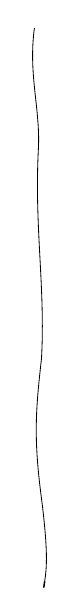
\begin{tikzpicture}[x=1cm,y=1cm,line cap=round]
\draw[line width=.30pt] (.03,0) .. controls (-.05,-.60) and (.11,-1.03) .. (.08,-1.55)
 .. controls (.03,-2.54) and (.17,-3.30) .. (.12,-4.20)
 .. controls (.04,-4.90) and (.02,-5.24) .. (.13,-6.05)
 .. controls (.20,-6.64) and (.19,-6.84) .. (.16,-7.03);
\draw[line width=.55pt] (.16,-7.03) -- (.15,-7.10);
\end{tikzpicture}}}
\unsure{Thus}; the datum of $u_0$
\deleted{\unsure{satisfying}} a loop \inserted{\unsure{outer automorphism}}
of $\widehat{\Pi}_{0,3}$ \unsure{commuting} with
$\mathfrak S_3$, or again
\unsure{an|$u$} outer automorphism of $\widehat{\mathfrak S}_{0,3}^{+}$
\unsure{inducing} the identity in $\mathfrak S_3$
and \deleted{\unsure{transforming}}
\inserted{\unsure{leaving invariant}} the conjugacy class
of the loop subgroup
$L'_0=\varepsilon_0^{\widehat{\mathbb Z}}={\ell'_0}^{\widehat{\mathbb Z}}
=\widehat{\varphi}(L_0)$,
or again that of a loop automorphism
$u_0$ of $\widehat{\Pi}_{0,3}$ \unsure{commuting} with
$\sigma_\infty$, and \unsure{in the outer automorphism quotien\textsuperscript{t}} with $\rho$,
or again of an automorphism $u$ of $\widehat{\mathfrak S}_{0,3}^{+}$
which fixes $\sigma_\infty$, and which fixes $\rho$ modulo $\widehat{\Pi}_{0,3}$
--- \unsure{is equivalent to} the datum of $g_0\in\widehat{\Pi}_{0,3}$ modulo $L_0$,
and of $\gamma\in\widehat{\mathbb Z}$, satisfying the relation

\scanpage{73}
\mspage{325}

\margin{\figure{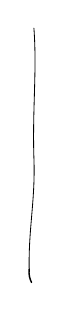
\begin{tikzpicture}[x=1cm,y=1cm,line cap=round]
\draw[line width=.30pt] (.04,0) .. controls (.08,-.55) and (.02,-1.02) .. (.04,-1.65)
 .. controls (.06,-2.18) and (-.03,-2.54) .. (-.02,-3.06);
\draw[line width=.52pt] (-.02,-3.06) .. controls (-.03,-3.13) and (-.01,-3.19) .. (.01,-3.23);
\end{tikzpicture}}}
\[
(38)\qquad \uline{g\rho(g)\rho^2(g)=1},
\]
where $g$ is given by (40), and where $u$ is expressed in terms of
\deleted{$g$} $g$ hence of $g_0,\gamma$ by
\[
(36)\qquad
\left\{\begin{aligned}
u(\sigma_\infty)&=\sigma_\infty\\
u(\rho)&=g\rho\qquad
\left(=\underbrace{\sigma_\infty(g_0)\ell_1^\gamma\rho(g_0)^{-1}}_g\rho\right).
\end{aligned}\right.
\]

\deleted{The relation (42)\inserted{\unsure{cf. = above}}, then reads,
since $L_0$ is generated by}
\[
\deleted{\ell_0=\underbrace{\ell'_0}_{\varepsilon_0}^{2}=(\sigma_\infty\rho)^2\deleted{\unsure{\sigma_\infty}}=\sigma_\infty\rho\sigma_\infty\rho}
\]
\[
\deleted{\underbrace{(u(\sigma_\infty\rho))}_{
\substack{\sigma_\infty g\rho=g_0\sigma_\infty \ell_1^\gamma\rho g_0^{-1}
=\operatorname{int}(g_0)(\sigma_\infty \ell_1^\gamma\rho)}}^{\unsure{2|4}}
\in\operatorname{int}(g_0)(\unsure{L'_0|L_0})\qquad\text{\unsure{now}}}
\]
\[
\deleted{\operatorname{int}(g_0)(\sigma_\infty \ell_1^\gamma\rho)^2\deleted{\unsure{g_0^{-1}}=1}}
\]
\deleted{thus (42) reads}
\[
\deleted{(\sigma_\infty \ell_1^\gamma\rho)^2\in L_0}
\]
\deleted{\unsure{i.e.}}
\[
\deleted{
\underbrace{\sigma_\infty \ell_1^\gamma\sigma_\infty}_{
    \underbrace{\sigma_\infty(\ell_1)}_{\ell_0}^{\gamma}}
  \underbrace{\sigma_\infty\illegible{1}\rho}_{\varepsilon_0}
}
\]
\margin{\deleted{N.B. $\operatorname{int}(g_0^{-1})u(\ell_0)$}}
\margin{\deleted{N.B. we have
$(\operatorname{int}(g_0^{-1})u)(\ell_0)
=(\sigma_\infty \ell_1^\gamma\rho)^2=\ell_0^{2\gamma+1}$}}
\deleted{\unsure{i.e.}}
\[
\deleted{\overset{\varepsilon_0^{2\gamma+1}}{\unsure{\ell_0^\gamma}\ \underbrace{\varepsilon_0}_{\unsure{\varepsilon_0^{2\gamma}}}}\in L_0}
\]
\deleted{therefore \unsure{\ldots}}
\[
\deleted{\unsure{\operatorname{int}(g_0)}\quad u(\ell_0)=}
\]

The relation (42), or the \unsure{apparently} stronger relation
\[
(43)\qquad u(L'_0)\subset\operatorname{int}(g_0)(L'_0)
\]
reads
\[
\underbrace{\operatorname{int}(g_0^{-1})\,
\underbrace{u(\underbrace{\sigma_\infty\rho}_{\ell'_0=\varepsilon_0})}_{
\sigma_\infty g\rho=g_0\sigma_\infty \ell_1^\gamma\rho g_0^{-1}}}_{
\sigma_\infty \ell_1^\gamma\rho
=\underbrace{\underbrace{\sigma_\infty \ell_1^\gamma\sigma_\infty}_{
 \underbrace{\sigma_\infty(\ell_1)^\gamma}_{\ell_0^\gamma=\varepsilon_0^{2\gamma}}}
\underbrace{\sigma_\infty\rho}_{\deleted{\unsure{\sigma_\infty\rho}}\varepsilon_0}}_{
\varepsilon_0^{2\gamma+1}}}
\in L'_0
\]
\margin{\uline{N.B.} we have
$\operatorname{int}(g_0^{-1})u(\underbrace{\ell'_0}_{\varepsilon_0})
=\varepsilon_0^{2\gamma+1}$}
\unsure{is satisfied} automatically, we \unsure{will have}
even
\[
\deleted{(44)\qquad u(\ell'_0)=u(\varepsilon_0)
=\operatorname{int}(g_0)(\ell'}
\]

\scanpage{74}

\[
(44)\qquad
u\bigl(\underset{\substack{\Vert\\ \varepsilon_0}}{\ell'_0}\bigr)
 = \operatorname{int}(g_0)\bigl(\underset{\substack{\Vert\\ \varepsilon_0}}{\ell'_0}{}^{p}\bigr)
\qquad \text{with}\quad \uuline{p=2\gamma+1}
\]
hence (39), \deleted{hence} on \unsure{raising} to the square:
\[
u(\ell_0)=\operatorname{int}(g_0)(\ell_0^p).
\]

\deleted{\unsure{We}}\quad
\uline{N.B.} We \unsure{will note} that if $p\in\widehat{\mathbb Z}^{*}$, then
$p-1\in 2\widehat{\mathbb Z}$ i.e.\ $\frac{p-1}{2}\in\widehat{\mathbb Z}$,
since it suffices to check the analogous relation for a $p\in\mathbb Z_\ell^{*}$,
\unsure{for|that} $p-1\in 2\mathbb Z_\ell$, now if $\ell\ne2$ we have
$2\mathbb Z_\ell=\mathbb Z_\ell$ OK, \unsure{there remains} the case $\ell=2$
$p\in\mathbb Z_2^{*}$ so the image of $p$ in $\mathbb Z/4\mathbb Z$
is $1$ or $3$ so $p-1\equiv0$ or $2\bmod4$
\deleted{\illegible{3}} so $\frac{p-1}{2}\in\mathbb Z_2$, OK.

\deleted{\unsure{It therefore remains to expri}}\par
It therefore remains to \unsure{express} condition (38), and we write it
\deleted{\unsure{in the form}}
\[
\underbrace{\sigma_\infty(g_0)\ell_1^\gamma\rho(g_0^{-1})}\,
\underbrace{\rho\sigma_\infty(g_0)\ell_\infty^\gamma\rho^2(g_0^{-1})}\,
\rho^2\sigma_\infty(g_0)\ell_0^\gamma g_0^{-1}=1
\]
i.e., on applying $\operatorname{int}(g_0^{-1})$ and
\deleted{\illegible{2}}\inserted{\unsure{setting again}}
(cf. (8))
\[
(45)\qquad g_0^{-1}\sigma_\infty(g_0)=h_0^{-1}
\qquad\text{i.e.}\quad
h_0=\sigma_\infty(g_0)^{-1}g_0=[\sigma_\infty,g_0^{-1}]
\]
\[
h_0^{-1}\ell_1^\gamma\underbrace{\rho(h_0^{-1})\ell_\infty^\gamma}\,
\rho^2(h_0^{-1})\ell_0^\gamma=1
\]
or again, on applying $\operatorname{int}(\ell_0^\gamma)$
\[
(46)\qquad
\boxed{\underbrace{(\ell_0^\gamma h_0^{-1})}\cdot
\rho(\ell_0^\gamma h_0^{-1})\cdot\rho^2(\ell_0^\gamma h_0^{-1})=1}
\qquad\left(\text{where }\gamma=\frac{p-1}{2}\right)
\]
which is none other than (10). As for the condition \unsure{(9)|(7)},
we see that it is \inserted{superfluous, i.e.,} automatically satisfied.

\scanpage{75}
\mspage{326}

Let us sum up:

\uline{Theorem} An outer automorphism\ \inserted{\unsure{with loops|with loops}} of
$\widehat{\Pi}_{0,3}$ commuting with
$\mathfrak S_3$, lifts uniquely as an automorphism
of the group \unsure{with loops|with loops} $\widehat{\Pi}_{0,3}$, commuting with
$\sigma_\infty$ (and commuting with $\rho$ modulo\ \unsure{inner|inner} automorphisms),
or again as the restriction of an automorphism\ $u$ of
$\widehat{\mathfrak S}_{0,3}^{+}$
which fixes $\sigma_\infty$, \unsure{leaves invariant} $\rho$ modulo $\widehat{\Pi}_{0,3}$
(i.e.\ \inserted{fixes} $\dot\rho$ in $\mathfrak S_3$),
and which \unsure{leaves invariant} the conjugacy class of the
\inserted{closed} subgroup $L'_0$\inserted{$=\widehat\varphi(L_0)$}
\deleted{\illegible{3}} generated by $\ell'_0=\varepsilon_0=\sigma_\infty\rho$.
(or again of the \inserted{closed} subgroup $L_0=(L'_0)^2$ generated by $\ell_0$).
The datum of such a $u$ is equivalent to that of its multiplier
$p\in\widehat{\mathbb Z}^{*}$, and of a $g_0\in\widehat{\Pi}_{0,3}/L_0$
satisfying the following conditions

 a) Setting
\[
(47)\qquad
\begin{cases}
h_0=\sigma_\infty(g_0)^{-1}g_0=[\sigma_\infty,g_0^{-1}]
   \quad(\in\widehat{\Pi}_{0,3})\\
\gamma=\dfrac{p-1}{2}\in\widehat{\mathbb Z}
\end{cases}
\]
we have relation (46) above (invariant under replacement of $g_0$ by
$g_0\ell_0^\lambda$, $\lambda\in\widehat{\mathbb Z}$)
\[
(48)\qquad
\bigl(\underbrace{\ell_0^\gamma h_0^{-1}}_{\xi_0}\bigr)
\rho(\ell_0^\gamma h_0^{-1})\rho^2(\ell_0^\gamma h_0^{-1})=1
\]
\margin{i.e.\ $\xi_0\rho(\xi_0)
\rho^{\unsure{2}}(\xi_0)=1$ with
$\xi_0=\ell_0^\gamma h_0^{-1}$}

 b) $\sigma_\infty$ and $g\rho$ generate \unsure{topologically}
$\widehat{\mathfrak S}_{0,3}^{+}$,
where $g$ is given in terms of $g_0$ by 40
\[
[(40)]\qquad
g=\sigma_\infty(g_0)\ell_1^\gamma\rho(g_0)^{-1}
=\sigma_\infty(g_0\ell_0^\gamma)\rho(g_0^{-1})
\]
\margin{$\begin{aligned}
&=g_0(h_0^{-1}\ell_1^\gamma)\rho(g_0)^{-1}\\
&=(g_0\ell_0^{-\gamma})(\ell_0^\gamma h_0^{-1})
  (\rho(g_0\ell_0^{-\gamma}))^{-1}
\end{aligned}$}

\deleted{\illegible{3}}
(\uline{N.B.} relation (46) is equivalent to:
\inserted{$(g\rho)^3=1$ i.e.\ to}
\[
(38)\qquad g\rho(g)\rho^2(g)=1,
\]
expressed directly in terms of $g_0$, $\gamma=\frac{p-1}{2}$),
with the generating relations $\sigma_\infty^2=(g\rho)^3=1$.
\margin{(36)}The automorphism\ $u$ is given in terms of $g_0$ and $p$ by

\scanpage{76}

\[
[(36)]\qquad
\begin{cases}
u(\sigma_\infty)=\sigma_\infty\\
u(\rho)=g\rho
\end{cases}
\qquad\text{where }g\text{ given by }[(40)])
\]

We will then have
\[
(49)\qquad
\begin{cases}
u(\ell_0)=\operatorname{int}(g_0)\ell_0^p\\
u(\ell_1)=\operatorname{int}(g_1)\ell_1^p
 \inserted{{}=\operatorname{int}(\sigma_\infty(g_0))(\ell_1^p)}\\
u(\ell_\infty)=\operatorname{int}(g_\infty)(\ell_\infty^p)
\end{cases}
\]
\margin{$\begin{aligned}
g_1&=g\rho(g_0)=\sigma_\infty(g_0)\ell_1^\gamma\\
   &=\sigma_\infty(g_0\ell_0^\gamma)\\
g_\infty&=g\rho(g_1)=\deleted{\unsure{g}}g\rho(g)\rho^2(g_0)\\
   &=\rho^2(g^{-1}g_0)=\rho(g_0\ell_0^\gamma)h_0
\end{aligned}$}

\margin{cf. \unsure{proposition} above}
\deleted{
\uline{Corollary} For the \unsure{surjective} homomorphism\ (18)
\[
\widehat\varphi:\widehat\Pi_{\unsure{0,3|3}}
\longrightarrow
\widehat{\mathfrak S}_{0,3}^{+}
\]
\deleted{\unsure{def}} defined by
\[
\ell_0\longmapsto \ell'_0=\sigma_\infty\rho,\quad
\ell_1\longmapsto \ell'_1=\sigma_\infty,\quad
\ell_\infty\longmapsto \ell'_\infty=\rho^{-1},
\]
to commute \inserted{up to inner automorphisms} with $u$, it is necessary and sufficient\ that we can
\unsure{find} $\beta\in\widehat{\mathbb Z}$ such that we have
\[
[(24)]\qquad
\varepsilon_1^{-\beta}h_0\varepsilon_0^\beta
=\sigma_\infty(\widehat\varphi(h_0))^{-1}\widehat\varphi(h_0)
\]
or what amounts to the same thing, that there exist
$\alpha\in\widehat{\mathbb Z}$ such that we have
\[
[(\unsure{30|38})]\qquad
\deleted{\unsure{h_0^{-1}}\ell_1^\gamma\rho
=\operatorname{int}(\varepsilon_0^\alpha\widehat\varphi(
\unsure{\rho^{-1}(h_0)|\rho^{-1}h_0)}))(\rho^p)}
\]
\deleted{$u(\rho)=\operatorname{int}($}
\[
h_0^{-1}\ell_1^\gamma\rho
=\operatorname{int}(\varepsilon_0^\alpha\widehat\varphi(
\unsure{\rho^{-1}(h_0)|\rho^{-1}h_0)}))(\rho^p)
\]
(where necessarily $\alpha=\beta+\gamma$).
}
\margin{$\beta$ \unsure{resp.} $\alpha$ are \unsure{uniquely} \unsure{determined}}

\scanpage{77}
\mspage{327}

\uline{\unsure{Scholium}} In the \unsure{theorem}, \unsure{the} $g$ \inserted{$\in\widehat{\Pi}_{0,3}$} (which \unsure{enters} directly in writing $u$) is expressed by means of the $g_0$ \inserted{$\in\widehat{\Pi}_{0,3}$} and $\gamma=\frac{p-1}{2}$, \deleted{\illegible{2}} ($g_0$ defined modulo $L_0$) --- condition (46) being in fact a condition which is expressed directly in terms of $g_0$, or better still, in terms of
\[
(50)\qquad
\xi_{\unsure{\deleted{0}|0}}=\ell_0^\gamma h_0^{-1}\in\widehat{\Pi}_{0,3}
\quad\text{(whence }h_0=\xi_{\unsure{\deleted{0}|0}}^{-1}\ell_0^\gamma\text{)}
\]
as
\[
(\unsure{51})\qquad \xi\rho(\xi)\rho^2(\xi)=1,
\]
which is equivalent to
\[
(52)\qquad (\xi\rho)^3=1.
\]

The solutions of equation (\unsure{51}), or what amounts to the same thing of (52), \unsure{correspond} to the splittings of \unsure{the|the} \inserted{\unsure{sub-}}extension \inserted{of $\widehat{\mathfrak S}_{0,3}^{+}$} of $\mathbb Z/3\mathbb Z$ by $\widehat{\Pi}_{0,3}$, \unsure{generated} by $\rho\in\mathfrak S_3$, \deleted{\illegible{1}} i.e. to the elements of order 3 of $\widehat{\mathfrak S}_{0,3}^{+}$ above $\dot\rho$.
On the set of these splittings resp. of these elements $\xi\rho$, $\widehat{\Pi}_{0,3}$ operates by inner automorphisms:
\[
(53)\qquad
\mathrm{int}(\lambda)(\xi\rho)
=\lambda\xi\rho\lambda^{-1}
=\lambda\xi\rho\lambda^{-1}\rho^{-1}\rho
=(\lambda\xi\rho(\lambda)^{-1})\rho
\]
i.e. it operates on the set of solutions of (\unsure{51}), by
\[
(54)\qquad {}^\lambda\xi=\lambda\xi\rho(\lambda)^{-1}
\]
\margin{\uline{N.B.} $\lambda\mapsto{}^\lambda\xi$ is injective}

\scanpage{78}

Let us admit (leaving it to be checked later) that there are exactly \unsure{two} conjugacy classes: that of $\xi_0=1$, corresponding to the tautological splitting, \deleted{\illegible{1}}\inserted{in} such a way that for such $\xi$ we will have
\[
(55)\qquad \xi=\lambda\rho(\lambda)^{-1}
\qquad(\lambda\in\widehat{\Pi}_{0,3}),
\]
and on the other hand the conjugacy class of the \unsure{lift$^{\mathrm t}$} of order 3 $\sigma_\infty\rho^{-1}\sigma_\infty^{-1}=\sigma_\infty\rho^{-1}\sigma_\infty$ of $\dot\rho$, corresponding to
\[
\sigma_\infty\rho^{-1}\sigma_\infty=\xi_0\rho,\quad\text{with}
\]
\[
\left\{\begin{aligned}
\xi_0&=\sigma_\infty\rho^{-1}\sigma_\infty\rho^{-1}
=\sigma_\infty\underbrace{(\rho^{-1}\sigma_\infty)}_{\varepsilon_0^{-1}}(\rho^{-1}\sigma_\infty)\sigma_\infty\\
&=\sigma_\infty\varepsilon_0^{-2}\deleted{\unsure{=}}\sigma_\infty
=\sigma_\infty(\ell_0^{-1})=\ell_1^{-1}
\end{aligned}\right.
\]
(and we do indeed have
\[
\ell_1^{-1}\rho(\ell_1^{-1})\rho^2(\ell_1^{-1})
=\ell_1^{-1}\ell_\infty^{-1}\ell_0^{-1}
=(\ell_0\ell_\infty\ell_1)^{-1}=1
\]
), This orbit corresponds to solutions of the form \deleted{\illegible{1}}
\[
(56)\qquad \xi=\lambda\ell_0^{-1}\rho(\lambda)^{-1}
\qquad(\lambda\in\widehat{\Pi}_{0,3})
\]
[we \unsure{will note} that $\ell_0^{-1}$ and $\ell_1^{-1}$ are in the same orbit
\[
\ell_1^{-1}=\deleted{\unsure{\ell_0\ell_1}\ \lambda\ell_1^{-1}\rho(\lambda)^{-1}}
\ell_0(\ell_0^{-1})\rho(\ell_0)^{-1}
\]
]

i.e. \deleted{$\ell_0=\rho(\lambda)\ell_1\lambda^{-1}$ \illegible{1} where $\lambda=\ell_\infty\ell_{\unsure{0}}$}

\deleted{Let us set}
\deleted{\unsure{a)}}

A) Case \deleted{\unsure{A}} where $\xi$ is of the form (55), hence
\[
(\unsure{56|57})\qquad h_0=\rho(\lambda)\lambda^{-1}\ell_0^\gamma
\]

\scanpage{79}
\mspage{328}

It remains then to solve the equation in $g_0$ (47)
\[
(58)\qquad
\sigma_\infty(g_0)^{-1}g_0
=\underbrace{\rho(\lambda)\lambda^{-1}\ell_0^\gamma}_{h_0}
\]
For \unsure{$\forall$|a} fixed $h_0$, there is at most a single $g_0$ which satisfies this condition, and such a $g_0$ exists \unsure{iff} \deleted{$\sigma_\infty(h_0)h_0=1$}, which is written
\margin{\unsure{using} \unsure{that} $\widehat{\Pi}_{0,3}^{\sigma_\infty}=\{1\}$}
\[
(59)\qquad \sigma_\infty(h_0)\cdot h_0=1
\qquad\inserted{\text{or again }h_0\sigma_\infty(h_0)=1}
\]
\deleted{$\sigma_\infty(\rho(\lambda))\sigma_\infty(\lambda^{-1})\ell_1^\gamma\rho(\lambda)\lambda^{-1}\ell_0^\gamma=1$}

which is also written, taking up again the expression $h_0=\xi^{-1}\ell_0^\gamma$
\[
\deleted{(\unsure{60})}\qquad
\sigma_\infty(\xi)^{-1}\ell_1^\gamma\xi^{-1}\ell_0^\gamma=1
\qquad\text{i.e.}
\]
\[
(60)\qquad \sigma_\infty(\xi)=\ell_1^\gamma\cdot\xi^{-1}\cdot\ell_0^\gamma
\]

In summary

\uline{Corollary} The $u$ which do not change the \inserted{$\widehat{\Pi}_{0,3}$-}conjugacy class of $\rho$ \deleted{are} correspond 1-1 to the systems $(\lambda,p)\in L_0\backslash\widehat{\Pi}_{0,3}\times\widehat{\mathbb Z}^{*}$, such that --- setting $\xi=\lambda\rho(\lambda)^{-1}$, \inserted{$\gamma=\frac{p-1}{2}$,} we have relation (60).
We will note that for $\lambda$ \unsure{hence} $\xi$ fixed, there exists at most \uuline{one} $\gamma\in\widehat{\mathbb Z}$ such that relation (60) holds, hence $p$ is determined by $\lambda$, subject to the \unsure{additional} condition that \inserted{the element} $2\gamma+1$ of $\widehat{\mathbb Z}$ be in $\widehat{\mathbb Z}^{*}$ (i.e. $\exists\gamma'\in\widehat{\mathbb Z}^{*}$ \unsure{with} $2\gamma\gamma'+\gamma+\gamma'=0$)

\scanpage{80}

\uline{N.B.} If $\lambda$ is replaced by $\lambda'=\ell_0^\alpha\lambda$, $\xi=\lambda\rho(\lambda)^{-1}$ is replaced by $\xi'=\ell_0^\alpha\cdot\xi\rho(\ell_0)^{-\alpha}$, and $h_0=\xi^{-1}\ell_0^\gamma$ is replaced by $h'_0=\rho(\ell_0)^\alpha h_0\ell_0^{-\alpha}$, finally $g_0$ is replaced by $g'_0=g_0\ell_0^{-\alpha}$, OK. \unsure{!} (Equation (60) for $\xi$ \unsure{or} for $\xi'$ is equivalent)

Finally, whether $u$ changes or does not change the $\widehat{\Pi}_{0,3}$-conjugacy class of $\rho$, the clearest approach for determining the $u$ in question seems to me to be this:

1$^\circ$) We choose a $\xi$ \inserted{$\in\widehat{\Pi}_{0,3}$} satisfying the equation
\[
(A)\qquad \xi\rho(\xi)\rho^2(\xi)=1
\]
(we \unsure{will take} it either in the form (55), or in the form (56)\deleted{\unsure{)}} :
\[
(B)\qquad
\xi=\lambda\rho(\lambda)^{-1}
\quad\text{or}\quad
\xi=\lambda\ell_0^{-1}\rho(\lambda)^{-1}
\quad\deleted{\unsure{\rbrace|\xi}},\quad\text{with }\lambda\in\widehat{\Pi}_{0,3}
\]
)

2$^\circ$) We choose $\gamma\in\widehat{\mathbb Z}$ such that
\[
(C)\qquad \sigma_\infty(\xi)=\ell_1^\gamma\xi^{-1}\ell_0^\gamma
\]
\margin{here, $\xi$ is \unsure{thus} given in terms of $\lambda$ \unsure{by by|by} (B)}
which determines $\gamma$ uniquely. We will in \unsure{1$^\circ$)|2$^\circ$)} have to restrict ourselves to the $\xi$ \inserted{(i.e. to the $\lambda$)} for which such a $\gamma$ exists, and such moreover that $p=2\gamma+1$ be $\in\widehat{\mathbb Z}^{*}$.
